\documentclass[border=6pt]{standalone}
\usepackage{tikz}
\usepackage{pgfplots}
\pgfplotsset{compat=1.18}
\usetikzlibrary{arrows.meta,positioning,shapes.geometric,fit,backgrounds,calc,decorations.pathreplacing,patterns,pgfplots.groupplots}
\tikzset{
  blk/.style={rectangle, rounded corners=2pt, draw=black!70, thick, fill=blue!6,
              minimum height=8mm, minimum width=20mm, align=center, font=\small},
  io/.style={rectangle, rounded corners=6pt, draw=black!70, thick, fill=green!8,
             minimum height=8mm, align=center, font=\small},
  proc/.style={rectangle, draw=black!70, thick, fill=orange!10, minimum height=8mm,
               align=center, font=\small},
  dec/.style={diamond, aspect=2, draw=black!70, thick, fill=yellow!15, align=center, font=\footnotesize},
  warnbox/.style={rectangle, rounded corners=2pt, draw=red!60!black, thick, fill=red!7,
                  minimum height=8mm, align=center, font=\small},
  oklbox/.style={rectangle, rounded corners=2pt, draw=green!45!black, thick, fill=green!8,
                 minimum height=8mm, align=center, font=\small},
  ar/.style={-{Latex[length=2mm]}, thick},
  arl/.style={-{Latex[length=2mm]}, thick, dashed, draw=black!55},
  lbl/.style={font=\footnotesize\itshape, text=black!60},
}
\definecolor{good}{RGB}{34,139,34}
\definecolor{bad}{RGB}{178,34,34}
\definecolor{warn}{RGB}{218,165,32}
\definecolor{pesblue}{RGB}{0,45,98}
\definecolor{complete}{RGB}{30,125,79}
\definecolor{partial}{RGB}{176,106,0}
\definecolor{blocked}{RGB}{166,43,43}
\begin{document}
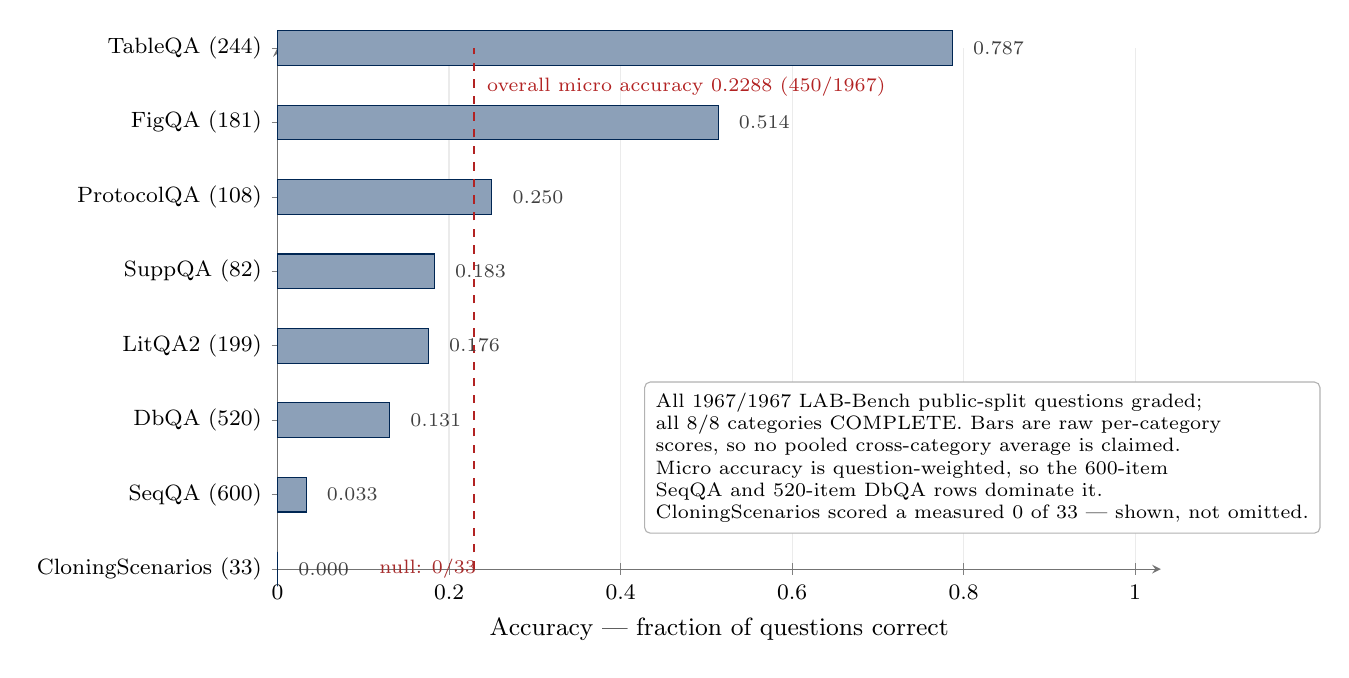
\begin{tikzpicture}
\begin{axis}[
    xbar,
    bar width=4.4mm,
    width=12.8cm,
    height=8.2cm,
    xmin=0,
    xmax=1.03,
    enlarge y limits={abs=0.62, upper},
    symbolic y coords={CloningScenarios,SeqQA,DbQA,LitQA2,SuppQA,ProtocolQA,FigQA,TableQA},
    ytick=data,
    yticklabels={CloningScenarios (33),SeqQA (600),DbQA (520),LitQA2 (199),SuppQA (82),ProtocolQA (108),FigQA (181),TableQA (244)},
    y tick label style={font=\footnotesize, align=right},
    x tick label style={font=\footnotesize},
    xtick={0,0.2,0.4,0.6,0.8,1.0},
    xlabel={Accuracy --- fraction of questions correct},
    xlabel style={font=\small},
    axis lines=left,
    axis line style={draw=black!55},
    xmajorgrids=true,
    grid style={draw=black!8},
    nodes near coords={\pgfmathprintnumber[fixed,fixed zerofill,precision=3]{\pgfplotspointmeta}},
    nodes near coords style={font=\scriptsize, anchor=west, xshift=1.4mm, text=black!75},
    clip=false,
]
\addplot[fill=pesblue!45, draw=pesblue!85!black] coordinates {
    (0.00000000000000000,CloningScenarios)
    (0.03333333333333333,SeqQA)
    (0.13076923076923078,DbQA)
    (0.17587939698492464,LitQA2)
    (0.18292682926829268,SuppQA)
    (0.25000000000000000,ProtocolQA)
    (0.51381215469613260,FigQA)
    (0.78688524590163930,TableQA)
};

% ---- overall micro (question-weighted) accuracy, all 1967 graded items ----
% x is placed at 0.2288/1.03 in relative axis coordinates so the symbolic
% y-axis is never asked to resolve a numeric y position.
\draw[bad, thick, dashed] (rel axis cs:0.22211,0) -- (rel axis cs:0.22211,1);
\node[font=\scriptsize, text=bad, anchor=south west, inner sep=1pt]
    at (rel axis cs:0.2335,0.900) {overall micro accuracy 0.2288 (450/1967)};

% ---- null result shown explicitly: zero bar is a real measured zero ----
\node[font=\scriptsize, text=blocked, anchor=west, inner sep=1pt]
    at (axis cs:0.115,CloningScenarios) {null: 0/33};

% ---- annotation block in the free lower-right region ----
\node[draw=black!30, rounded corners=2pt, fill=white, font=\scriptsize,
      align=left, inner sep=4pt, anchor=north west]
    at (rel axis cs:0.415,0.360) {%
      All 1967/1967 LAB-Bench public-split questions graded;\\
      all 8/8 categories COMPLETE. Bars are raw per-category\\
      scores, so no pooled cross-category average is claimed.\\
      Micro accuracy is question-weighted, so the 600-item\\
      SeqQA and 520-item DbQA rows dominate it.\\
      CloningScenarios scored a measured 0 of 33 --- shown, not omitted.};
\end{axis}
\end{tikzpicture}
\end{document}
